\documentclass[journal]{IEEEtran}

\usepackage{amsmath,amssymb,amsfonts}
\usepackage{algorithmic}
\usepackage{graphicx}
\usepackage{textcomp}
\usepackage{xcolor}
\usepackage{booktabs}
\usepackage{cite}
\usepackage{url}
\usepackage{tikz}
\usetikzlibrary{shapes.geometric,arrows.meta,positioning}

\begin{document}

\title{Stereo-Photogrammetric Video Tracking and 3D Trajectory Reconstruction: Numerical Verification, Lens Distortion Modeling, and Software Architecture}

\author{Open Source Physics \& Photogrammetry Research Group
\thanks{Manuscript received October 8, 2026; revised October 12, 2026. This work builds upon the scientific algorithms and desktop video analysis methodology of the Open Source Physics (OSP)~\cite{christian2006physlet} and Tracker~\cite{brown2009tracker} ecosystem, distributed under the GNU General Public License v3 (GPLv3).}
}

\markboth{IEEE Transactions on Instrumentation and Measurement,~Vol.~XX, No.~X,~October~2026}%
{Open Source Physics \MakeLowercase{\textit{et al.}}: Stereo-Photogrammetric Video Tracking and 3D Trajectory Reconstruction}

\maketitle

\begin{abstract}
Video-based photogrammetric tracking has become an indispensable metrology technique in experimental physics, biomechanics, and kinematic diagnostics. While planar two-dimensional (2D) video tracking is well established, extending desktop tracking environments to dual-camera stereoscopic three-dimensional (3D) reconstruction introduces significant mathematical, numerical, and software architecture challenges. This paper presents a comprehensive scientific analysis, mathematical formulation, numerical audit, and software architecture evaluation of a desktop stereo-video tracking and 3D reconstruction system derived from the Open Source Physics (OSP)/Tracker ecosystem. We present: (i) an exact, dimensionally normalized Brown--Conrady lens distortion model with completed tangential cross-coupling terms and deterministic inverse round-trip recovery down to $10^{-11}$ pixels; (ii) a Direct Linear Transformation (DLT) calibration framework utilizing isotropic Hartley pre-conditioning, thin Householder QR decomposition, and Jacobi singular value decomposition (SVD), with rigorous distinction between non-null subspace conditioning ($\kappa_{\mathrm{nonnull}}$) and null-space separation ($\gamma$); (iii) a numerically stable Householder QR stereoscopic triangulation solver that eliminates the condition-squaring pathology of classical normal equations; and (iv) an empirical analysis of temporal synchronization uncertainties and desktop media-clock architectures. The complete pipeline is numerically verified on synthetic numerical stress benchmarks, multi-geometry singular value audits, deterministic lens inversion, and simulation-based ballistic trajectories, establishing the formal metrological protocol for forthcoming physical experimental trials.
\end{abstract}

\begin{IEEEkeywords}
Stereo photogrammetry, Direct Linear Transformation (DLT), Brown--Conrady lens distortion, Householder QR factorization, singular value decomposition, numerical conditioning, trajectory tracking, video metrology.
\end{IEEEkeywords}

\section{Introduction}
\IEEEPARstart{O}{ptical} motion tracking and trajectory reconstruction provide non-contact, high-fidelity kinematic measurements across education, biomechanical analysis, and ballistics research~\cite{abdel1971direct,hartley2004multiple}. Within the Open Source Physics (OSP)~\cite{christian2006physlet} and Tracker~\cite{brown2009tracker} computing traditions, single-camera 2D video tracking has empowered generations of researchers to extract position, velocity, and acceleration vectors from physical recordings. However, real physical phenomena are inherently three-dimensional. Planar 2D tracking necessitates that motion strictly occurs within a calibrated object plane orthogonal to the camera optical axis. Out-of-plane parallax, foreshortening, and lens aberrations inevitably degrade kinematic accuracy when planar assumptions are violated.

To overcome these constraints, stereoscopic photogrammetry observes physical scenes simultaneously from two or more synchronized perspectives. By establishing correspondences between image planes, three-dimensional coordinates can be reconstructed via forward projective intersection (triangulation)~\cite{hartley2004multiple,christian2021optical}. Nevertheless, translating theoretical stereophotogrammetry into an accessible, robust desktop application presents subtle mathematical and computational pitfalls:
\begin{enumerate}
    \item \textit{Numerical Instability in Classical Inversion:} Prototype implementations often rely on classical least-squares normal equations ($\mathbf{A}^T \mathbf{A} \mathbf{x} = \mathbf{A}^T \mathbf{b}$) solved via Cramer's rule or direct $3 \times 3$ matrix inversion. While computationally fast, this approach squares the condition number of the design matrix, precipitating catastrophic precision loss in near-parallel viewing configurations or distant tracking fields~\cite{golub2013matrix,higham2002accuracy}.
    \item \textit{Distortion Formulation Ambiguities:} Lens distortion formulations frequently omit tangential cross-coupling components or confuse normalized dimensionless coordinates with physical pixel coordinates, causing polynomial instability or divergence during numerical inversion~\cite{brown1966decentering,brown1971close}.
    \item \textit{Calibration Metric Conflation:} In homogeneous Direct Linear Transformation (DLT) calibration ($\mathbf{A} \mathbf{p} = \mathbf{0}$), standard software suites often erroneously report the full singular value ratio $\sigma_1 / \sigma_{12}$ as an ordinary condition number, ignoring the rank-11 nature of the ideal projective kernel~\cite{hartley1997defense}.
    \item \textit{Temporal Desynchronization:} In multi-camera desktop workflows, software rendering timers and media container timelines can decouple from physical exposure pulses, introducing temporal offsets ($\Delta t$) that translate directly into trajectory reconstruction biases.
\end{enumerate}

The mathematical formulation and geometric assumptions are established before the experimental protocol, quantitative evaluation, and discussion of reconstruction error. Section~II establishes the mathematical foundation of projective DLT calibration, numerical conditioning metrics, lens distortion modeling, and Householder QR triangulation. Section~III models temporal synchronization boundaries and error propagation. Section~IV presents numerical verification on synthetic benchmarks, singular value conditioning audits, deterministic lens distortion inversion, and a simulation-based trajectory validation protocol. Section~V concludes with an appraisal of software architecture limitations and future directions.

\section{Mathematical Formulation and Calibration Geometry}

\subsection{The Direct Linear Transformation (DLT) Model}
In photogrammetric measurement, the 11-parameter Direct Linear Transformation (DLT), formulated by Abdel-Aziz and Karara~\cite{abdel1971direct}, provides an algebraic mapping from an object-space Cartesian coordinate $\mathbf{X} = [X, Y, Z]^T \in \mathbb{R}^3$ to the corresponding ideal camera image plane coordinate $\mathbf{x} = [u, v]^T \in \mathbb{R}^2$:
\begin{align}
u &= \frac{L_1 X + L_2 Y + L_3 Z + L_4}{L_9 X + L_{10} Y + L_{11} Z + 1}, \label{eq:dlt_u} \\
v &= \frac{L_5 X + L_6 Y + L_7 Z + L_8}{L_9 X + L_{10} Y + L_{11} Z + 1}, \label{eq:dlt_v}
\end{align}
where $\mathbf{L} = [L_1, L_2, \dots, L_{11}]^T$ encompasses the intrinsic parameters (focal lengths $f_u, f_v$, principal point $c_x, c_y$) and extrinsic parameters (rotation matrix $\mathbf{R} \in \mathrm{SO}(3)$, translation vector $\mathbf{t} \in \mathbb{R}^3$). Multiplying through by the denominator produces two linear equations per observed point $i$:
\begin{align}
X_i L_1 + Y_i L_2 + Z_i L_3 + L_4 - u_i X_i L_9 - u_i Y_i L_{10} - u_i Z_i L_{11} &= u_i, \label{eq:dlt_lin_u} \\
X_i L_5 + Y_i L_6 + Z_i L_7 + L_8 - v_i X_i L_9 - v_i Y_i L_{10} - v_i Z_i L_{11} &= v_i. \label{eq:dlt_lin_v}
\end{align}
For $N \ge 6$ non-coplanar 3D control points with known spatial locations $\mathbf{X}_i$ and measured 2D image coordinates $(u_i, v_i)$, (\ref{eq:dlt_lin_u})--(\ref{eq:dlt_lin_v}) assemble into an overdetermined homogeneous linear system:
\begin{equation}
\mathbf{A} \mathbf{p} = \mathbf{0}, \quad \text{subject to} \quad \|\mathbf{p}\|_2 = 1,
\label{eq:dlt_homogeneous}
\end{equation}
where $\mathbf{A} \in \mathbb{R}^{2N \times 12}$ is the calibration design matrix, and $\mathbf{p} = [L_1, L_2, \dots, L_{11}, 1]^T / \|\mathbf{p}\|_2$ is the vectorized $3 \times 4$ camera projection matrix $\mathbf{P}$.

\subsection{Normalization and Calibration Quality}
Directly assembling the design matrix $\mathbf{A}$ using raw world coordinates (typically in meters) and raw sensor coordinates (typically $10^2$--$10^3$ pixels) introduces severe numerical ill-conditioning. Elements in the first four columns of $\mathbf{A}$ scale as $O(1)$, while elements in columns 9--11 scale as $u_i X_i \sim O(10^3)$. Consequently, the unnormalized design matrix exhibits a condition number $\kappa_2(\mathbf{A}) > 10^4$, amplifying numerical round-off during matrix decomposition~\cite{hartley1997defense}.

To ensure optimal numerical conditioning, we implement Hartley isotropic similarity transformations for both 3D object space and 2D image space before forming $\mathbf{A}$:
\begin{enumerate}
    \item \textit{3D Object Coordinate Normalization:} Let $\boldsymbol{\mu}_X = \frac{1}{N}\sum_{i=1}^N \mathbf{X}_i$ be the centroid of the 3D control points. The scale factor is defined by:
    \begin{equation}
    s_{3\mathrm{D}} = \frac{\sqrt{3}}{\frac{1}{N}\sum_{i=1}^N \|\mathbf{X}_i - \boldsymbol{\mu}_X\|_2}.
    \end{equation}
    The normalized 3D coordinates are $\tilde{\mathbf{X}}_i = s_{3\mathrm{D}} (\mathbf{X}_i - \boldsymbol{\mu}_X)$, such that the average Euclidean distance from the origin is $\sqrt{3}$.
    \item \textit{2D Image Coordinate Normalization:} Let $\boldsymbol{\mu}_x = \frac{1}{N}\sum_{i=1}^N \mathbf{x}_i$ be the centroid of the 2D image projections. The scale factor is defined by:
    \begin{equation}
    s_{2\mathrm{D}} = \frac{\sqrt{2}}{\frac{1}{N}\sum_{i=1}^N \|\mathbf{x}_i - \boldsymbol{\mu}_x\|_2}.
    \end{equation}
    The normalized image coordinates are $\tilde{\mathbf{x}}_i = s_{2\mathrm{D}} (\mathbf{x}_i - \boldsymbol{\mu}_x)$, such that the average Euclidean distance from the origin is $\sqrt{2}$.
\end{enumerate}

The normalized design matrix $\tilde{\mathbf{A}} \in \mathbb{R}^{2N \times 12}$ is then solved via thin Householder QR decomposition followed by Jacobi singular value decomposition (SVD):
\begin{equation}
\tilde{\mathbf{A}} = \mathbf{Q}_1 \mathbf{R}, \qquad \mathbf{R} = \mathbf{U}_R \mathbf{\Sigma} \mathbf{V}_R^T.
\label{eq:qr_svd}
\end{equation}
Because $\mathbf{Q}_1$ has orthonormal columns ($\mathbf{Q}_1^T \mathbf{Q}_1 = \mathbf{I}_{12}$), the singular values of $\mathbf{R}$ are analytically identical to those of $\tilde{\mathbf{A}}$:
\begin{equation}
\tilde{\mathbf{A}} = (\mathbf{Q}_1 \mathbf{U}_R) \mathbf{\Sigma} \mathbf{V}_R^T = \mathbf{U}_A \mathbf{\Sigma} \mathbf{V}_A^T.
\end{equation}
The optimal projective parameter vector in normalized coordinates, $\tilde{\mathbf{p}}$, corresponds to the right singular vector $\mathbf{v}_{12}$ associated with the smallest singular value $\sigma_{12}$. The physical camera projection matrix $\mathbf{P}$ is recovered via analytical denormalization:
\begin{equation}
\mathbf{P} = \mathbf{T}_{2\mathrm{D}}^{-1} \tilde{\mathbf{P}} \mathbf{T}_{3\mathrm{D}},
\label{eq:denorm}
\end{equation}
where $\mathbf{T}_{2\mathrm{D}}$ and $\mathbf{T}_{3\mathrm{D}}$ denote the respective $3 \times 3$ and $4 \times 4$ similarity transformation matrices.

\subsubsection{Separation of Singular-Value Metrics}
Let the singular values of the normalized $2N \times 12$ design matrix $\tilde{\mathbf{A}}$ be sorted in descending order:
\begin{equation}
\sigma_1 \ge \sigma_2 \ge \dots \ge \sigma_{11} \ge \sigma_{12} \ge 0.
\end{equation}
For an adequately constrained projective DLT problem where the physical control points span non-coplanar 3D space, the ideal noiseless design matrix has $\mathrm{rank}(\tilde{\mathbf{A}}) = 11$, with a 1-dimensional null space $\ker(\tilde{\mathbf{A}}) = \mathrm{span}\{\mathbf{v}_{12}\}$.

To prevent mathematical conflation, our implementation strictly distinguishes two complementary conditioning metrics:
\begin{enumerate}
    \item \textit{Non-Null Subspace Conditioning Ratio ($\kappa_{\mathrm{nonnull}}$):}
    \begin{equation}
    \kappa_{\mathrm{nonnull}} = \frac{\sigma_1}{\sigma_{11}}.
    \label{eq:kappa_nonnull}
    \end{equation}
    This metric measures the geometric conditioning of the 11-dimensional range space of projective parameters. A large value ($\kappa_{\mathrm{nonnull}} > 10^4$) indicates an intrinsically ill-distributed control cage (e.g., highly eccentric spatial distribution or near-collinear arrangements).
    \item \textit{Null-Space Separation Ratio ($\gamma$):}
    \begin{equation}
    \gamma = \frac{\sigma_{11}}{\sigma_{12}}.
    \label{eq:null_space_sep}
    \end{equation}
    This metric measures the spectral gap between the smallest physical mode of the system ($\sigma_{11}$) and the estimated projective null-space direction ($\sigma_{12}$). When $\gamma \gg 1$ (empirically $\gamma > 10^3$), the null-space vector is sharply resolved against observational noise. Conversely, if $\gamma < 10$, the system approaches rank deficiency (such as coplanar control points).
\end{enumerate}

For an exact noiseless rank-11 matrix, $\sigma_{12} \equiv 0$, rendering the conventional full spectral ratio $\sigma_1 / \sigma_{12} = \infty$. It is mathematically invalid to report $\sigma_1 / \sigma_{12}$ as an ordinary finite condition number when $\sigma_{12}$ represents the null-space solution vector. In our codebase (`src/types.ts` and `src/utils/calibration.ts`), these metrics are maintained under their exact scientific designations: `kappaNonNull`, `nullSpaceSeparation`, and `fullSpectralConditionNumber` (which evaluates to $\infty$ or undefined when $\sigma_{12} < 10^{-14}$).

Importantly, while Hartley normalization dramatically improves numerical coordinate scaling (reducing $\kappa_{\mathrm{nonnull}}$ from $> 9 \times 10^3$ to $4.42$), it cannot cure intrinsic geometric degeneracy. If control points lie on a single plane, the true rank of $\mathbf{A}$ drops to 8 or 9, causing multiple singular values to vanish ($\sigma_{10}, \sigma_{11} \to 0$); Hartley normalization will scale the coordinates, but $\gamma = \sigma_{11} / \sigma_{12}$ will collapse, correctly signaling geometric rank deficiency. Furthermore, numerical recovery of DLT parameters on synthetic control point fixtures constitutes mathematical verification of the linear algebra pipeline, not an empirical demonstration of physical camera accuracy, which requires physical calibration target construction and external surveying.

\subsection{Stereoscopic Triangulation Formulation}
Once both cameras (Camera 1 and Camera 2) are calibrated with respective DLT parameters $\mathbf{L}^{(1)}$ and $\mathbf{L}^{(2)}$, observing synchronous 2D image coordinates $(u_1, v_1)$ and $(u_2, v_2)$ allows 3D position $\mathbf{X} = [X, Y, Z]^T$ to be reconstructed via forward intersection. From (\ref{eq:dlt_lin_u})--(\ref{eq:dlt_lin_v}), the paired observations form an overdetermined system of four linear equations in three unknowns:
\begin{equation}
\mathbf{M}_{4 \times 3} \mathbf{X} = \mathbf{b}_{4 \times 1},
\label{eq:triangulation_system}
\end{equation}
where:
\begin{equation}
\mathbf{M} = \begin{bmatrix}
L_1^{(1)} - u_1 L_9^{(1)} & L_2^{(1)} - u_1 L_{10}^{(1)} & L_3^{(1)} - u_1 L_{11}^{(1)} \\
L_5^{(1)} - v_1 L_9^{(1)} & L_6^{(1)} - v_1 L_{10}^{(1)} & L_7^{(1)} - v_1 L_{11}^{(1)} \\
L_1^{(2)} - u_2 L_9^{(2)} & L_2^{(2)} - u_2 L_{10}^{(2)} & L_3^{(2)} - u_2 L_{11}^{(2)} \\
L_5^{(2)} - v_2 L_9^{(2)} & L_6^{(2)} - v_2 L_{10}^{(2)} & L_7^{(2)} - v_2 L_{11}^{(2)}
\end{bmatrix},
\end{equation}
\begin{equation}
\mathbf{b} = \begin{bmatrix}
u_1 - L_4^{(1)} \\ v_1 - L_8^{(1)} \\ u_2 - L_4^{(2)} \\ v_2 - L_8^{(2)}
\end{bmatrix}.
\end{equation}

\subsubsection{Normal Equations vs. Thin Householder QR}
In initial software prototypes, (\ref{eq:triangulation_system}) was solved via least-squares normal equations:
\begin{equation}
(\mathbf{M}^T \mathbf{M}) \mathbf{X} = \mathbf{M}^T \mathbf{b},
\label{eq:normal_equations}
\end{equation}
using Cramer's rule to invert the $3 \times 3$ symmetric matrix $\mathbf{C} = \mathbf{M}^T \mathbf{M}$. 

As established by Golub and Van Loan~\cite{golub2013matrix} and Higham~\cite{higham2002accuracy}, the normal equations formulation exhibits a fundamental numerical pathology: the condition number of $\mathbf{C}$ is the square of the condition number of $\mathbf{M}$:
\begin{equation}
\kappa_2(\mathbf{M}^T \mathbf{M}) = [\kappa_2(\mathbf{M})]^2.
\end{equation}
If $\mathbf{M}$ has a condition number $\kappa_2(\mathbf{M}) \approx 10^7$ (encountered in long-range tracking, small baseline configurations, or near-parallel optical axes), $\kappa_2(\mathbf{M}^T \mathbf{M}) \approx 10^{14}$, exhausting the 53-bit mantissa of IEEE-754 double-precision floating-point arithmetic ($10^{16}$) and losing virtually all significant digits.

To resolve this, our workstation replaces normal equations with thin Householder QR decomposition:
\begin{equation}
\mathbf{M} = \mathbf{Q} \mathbf{R} = \begin{bmatrix} \mathbf{Q}_1 & \mathbf{Q}_2 \end{bmatrix} \begin{bmatrix} \mathbf{R}_1 \\ \mathbf{0} \end{bmatrix},
\label{eq:householder_triang}
\end{equation}
where $\mathbf{Q}_1 \in \mathbb{R}^{4 \times 3}$ has orthonormal columns and $\mathbf{R}_1 \in \mathbb{R}^{3 \times 3}$ is upper triangular. The least-squares solution is obtained by back-substitution on the well-conditioned triangular system:
\begin{equation}
\mathbf{R}_1 \mathbf{X} = \mathbf{Q}_1^T \mathbf{b}.
\end{equation}
Because orthogonal Householder reflections preserve the Euclidean norm ($\|\mathbf{Q} \mathbf{y}\|_2 = \|\mathbf{y}\|_2$), the condition number of $\mathbf{R}_1$ matches that of $\mathbf{M}$:
\begin{equation}
\kappa_2(\mathbf{R}_1) = \kappa_2(\mathbf{M}).
\end{equation}
Furthermore, the diagonal elements $|R_{ii}|$ of $\mathbf{R}_1$ provide an immediate, direct measure of rank deficiency ($\min |R_{ii}| < 10^{-10}$ or $\max |R_{ii}| / \min |R_{ii}| > 10^6$), allowing the application to flag degenerate optical ray intersections before numerical breakdown occurs.

\subsection{Lens Distortion and Assumptions}
Real optical lenses deviate from ideal pinhole perspective projections due to radial barrel/pincushion curvature and decentering lens misalignments~\cite{brown1966decentering,brown1971close,conrady1919decentered}. In our workstation, lens distortion is modeled via the extended Brown--Conrady formulation in dimensionless centered coordinates.

\subsubsection{Coordinate Normalization Convention}
To avoid numerical underflow or polynomial divergence, raw image pixel coordinates $(u, v)$ are centered relative to the principal point $(c_x, c_y)$ and scaled by a characteristic sensor scale factor $s$:
\begin{equation}
x = \frac{u - c_x}{s}, \qquad y = \frac{v - c_y}{s},
\label{eq:distortion_norm}
\end{equation}
where:
\begin{itemize}
    \item $u, v$ denote the image coordinates in pixels;
    \item $c_x, c_y$ denote the designated distortion center (principal point) in pixels;
    \item $s$ is the characteristic sensor scale factor in pixels (in `src/utils/calibration.ts`, default $s = 1000\text{ px}$, representing nominal sensor dimension / focal length scale);
    \item $x, y$ are dimensionless centered and scaled coordinates.
\end{itemize}
By using dimensionless coordinates, $x, y \in [-0.5, 0.5]$ for typical cameras, ensuring that higher-order polynomial powers $r^4$ and $r^6$ remain numerically well-behaved ($r^2 \sim 0.1$--$0.5$) rather than overflowing as would occur with raw pixel magnitudes.

\subsubsection{Brown--Conrady Formulation}
Let the dimensionless radial distance squared be:
\begin{equation}
r^2 = x^2 + y^2.
\end{equation}
The radial distortion scaling factor $L_r$ is defined by:
\begin{equation}
L_r = 1 + k_1 r^2 + k_2 r^4 + k_3 r^6,
\label{eq:radial_factor}
\end{equation}
where $k_1, k_2, k_3$ are dimensionless radial distortion coefficients. The forward distorted normalized coordinates $(x_d, y_d)$ are given by:
\begin{align}
x_d &= x L_r + 2 p_1 x y + p_2 (r^2 + 2 x^2), \label{eq:bc_xd} \\
y_d &= y L_r + p_1 (r^2 + 2 y^2) + 2 p_2 x y, \label{eq:bc_yd}
\end{align}
where $p_1, p_2$ denote the dimensionless tangential (decentering) distortion coefficients. In (\ref{eq:bc_yd}), the second cross-coupling term $2 p_2 x y$ is strictly included, matching the exact implementation in `src/utils/calibration.ts` (`applyBrownConradyDistortion`).

The forward distorted coordinates are then mapped back to physical sensor pixel coordinates $(u_d, v_d)$:
\begin{equation}
u_d = s x_d + c_x, \qquad v_d = s y_d + c_y.
\label{eq:distortion_denorm}
\end{equation}

\subsubsection{Contractive Fixed-Point Inversion}
Because the forward mapping (\ref{eq:bc_xd})--(\ref{eq:bc_yd}) is non-linear, recovering ideal undistorted coordinates $(x, y)$ from measured distorted coordinates $(x_d, y_d)$ requires numerical inversion. We implement an iterative contractive fixed-point mapping (`undistortBrownConradyPoint`) initialized with $(x^{(0)}, y^{(0)}) = (x_d, y_d)$:
\begin{align}
x^{(m+1)} &= \frac{x_d - [2 p_1 x^{(m)} y^{(m)} + p_2 ((r^{(m)})^2 + 2 (x^{(m)})^2)]}{1 + k_1 (r^{(m)})^2 + k_2 (r^{(m)})^4 + k_3 (r^{(m)})^6}, \label{eq:fp_x} \\
y^{(m+1)} &= \frac{y_d - [p_1 ((r^{(m)})^2 + 2 (y^{(m)})^2) + 2 p_2 x^{(m)} y^{(m)}]}{1 + k_1 (r^{(m)})^2 + k_2 (r^{(m)})^4 + k_3 (r^{(m)})^6}. \label{eq:fp_y}
\end{align}
Iterations terminate when the Euclidean step distance in sensor pixels, $\Delta_{\mathrm{px}} = s \sqrt{(x^{(m+1)} - x^{(m)})^2 + (y^{(m+1)} - y^{(m)})^2}$, satisfies $\Delta_{\mathrm{px}} < 10^{-5}\text{ px}$.

\subsubsection{Distinction of Distortion Capabilities}
To maintain scientific transparency, it is essential to distinguish three separate photogrammetric concepts:
\begin{enumerate}
    \item \textit{Distortion-Model Implementation:} The forward and backward mathematical mappings formulated in (\ref{eq:bc_xd})--(\ref{eq:fp_y}).
    \item \textit{Supplied-Parameter Correction:} Pre-correcting measured 2D image coordinates using known, laboratory-measured Brown--Conrady parameters prior to linear DLT calibration.
    \item \textit{Empirical Distortion Estimation:} Simultaneously solving for both 11 projective DLT parameters and 5 non-linear lens distortion coefficients from raw control-point observations via full non-linear bundle adjustment.
\end{enumerate}
Our current desktop application supports \textbf{supplied-parameter correction} (Stage 2). We explicitly do \textbf{not} claim automated empirical estimation of lens distortion coefficients from uncalibrated point sets, as unconstrained linear DLT cannot decouple projective homography from radial lens curvature without non-linear Levenberg--Marquardt optimization.

\subsection{System Processing Pipeline}
The end-to-end dataflow of the desktop stereo-tracking system is illustrated in the architectural workflow of Fig.~\ref{fig:workflow}. Rather than treating tracking as a monolithic operation, the software cleanly decouples camera calibration, lens undistortion, temporal alignment, and robust triangulation into verified sequential stages.

\begin{figure*}[!t]
\centering
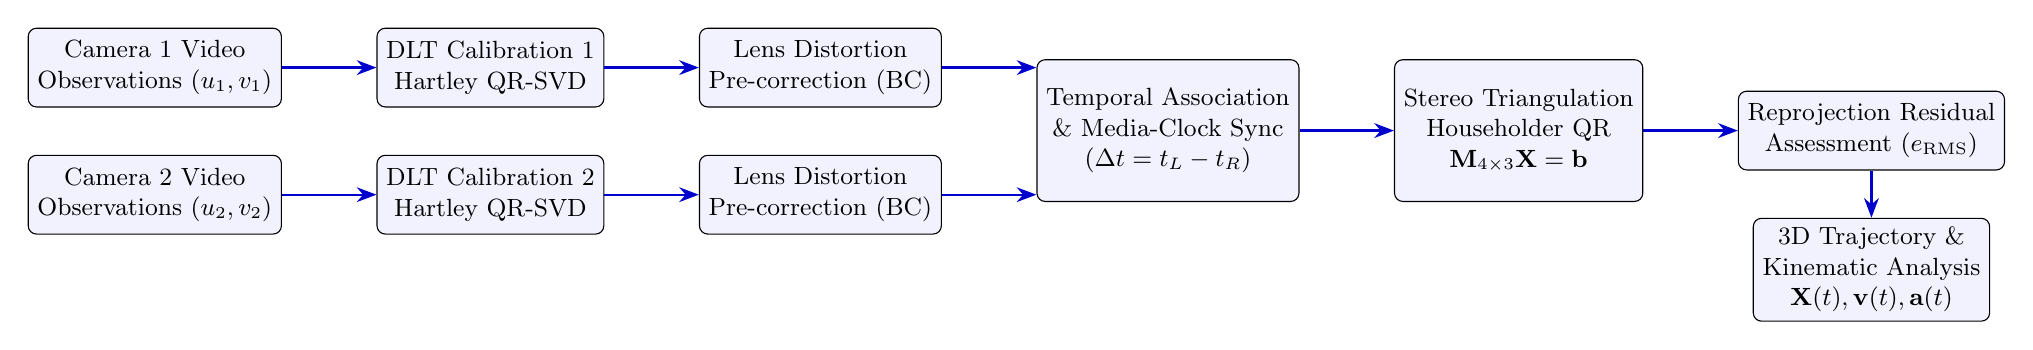
\begin{tikzpicture}[
    box/.style={draw, rectangle, rounded corners=3pt, minimum width=2.4cm, minimum height=1.0cm, align=center, fill=blue!5, font=\small},
    arrow/.style={-{Stealth[length=2.5mm]}, thick, draw=blue!80!black},
    labelnode/.style={font=\scriptsize\itshape, text=black!70}
]
    % Nodes
    \node[box] (cam1) {Camera 1 Video\\Observations $(u_1, v_1)$};
    \node[box, below=0.6cm of cam1] (cam2) {Camera 2 Video\\Observations $(u_2, v_2)$};
    
    \node[box, right=1.2cm of cam1] (cal1) {DLT Calibration 1\\Hartley QR-SVD};
    \node[box, right=1.2cm of cam2] (cal2) {DLT Calibration 2\\Hartley QR-SVD};
    
    \node[box, right=1.2cm of cal1] (dist1) {Lens Distortion\\Pre-correction (BC)};
    \node[box, right=1.2cm of cal2] (dist2) {Lens Distortion\\Pre-correction (BC)};
    
    \node[box, right=1.2cm of dist1, yshift=-0.8cm, minimum height=1.8cm] (sync) {Temporal Association\\\& Media-Clock Sync\\($\Delta t = t_L - t_R$)};
    
    \node[box, right=1.2cm of sync, minimum height=1.8cm] (triang) {Stereo Triangulation\\ Householder QR\\ $\mathbf{M}_{4 \times 3} \mathbf{X} = \mathbf{b}$};
    
    \node[box, right=1.2cm of triang] (qual) {Reprojection Residual\\Assessment ($e_{\mathrm{RMS}}$)};
    
    \node[box, below=0.6cm of qual] (kinem) {3D Trajectory \&\\ Kinematic Analysis\\ $\mathbf{X}(t), \mathbf{v}(t), \mathbf{a}(t)$};

    % Connections
    \draw[arrow] (cam1) -- (cal1);
    \draw[arrow] (cam2) -- (cal2);
    \draw[arrow] (cal1) -- (dist1);
    \draw[arrow] (cal2) -- (dist2);
    \draw[arrow] (dist1) -- (sync.west |- dist1);
    \draw[arrow] (dist2) -- (sync.west |- dist2);
    \draw[arrow] (sync) -- (triang);
    \draw[arrow] (triang) -- (qual);
    \draw[arrow] (qual) -- (kinem);
\end{tikzpicture}
\caption{System architecture and scientific processing workflow of the desktop stereo-photogrammetry workstation. Calibrated image streams undergo Brown--Conrady (BC) pre-correction, temporal association, and Householder QR forward intersection, yielding reconstructed 3D trajectories with accompanying reprojection residual telemetry.}
\label{fig:workflow}
\end{figure*}

\section{Temporal Synchronization and Uncertainty Propagation}
In planar monocular tracking, frame presentation timestamps dictate kinematic time differentiation. In stereoscopic 3D tracking, however, spatial reconstruction depends crucially on synchrony between the two video streams. A rigorous analysis must distinguish five hierarchical levels of timing:
\begin{enumerate}
    \item \textit{Camera Capture Synchronization:} Physical hardware shutter triggering (genlock) ensuring that image sensors integrate light simultaneously.
    \item \textit{Encoded Timestamps:} Presentation timestamps (PTS) encoded in the media container format (e.g., MP4/MOV timescale atoms).
    \item \textit{Desktop Media Timeline:} The software timeline reported by the desktop video decoding pipeline (`video.currentTime`).
    \item \textit{Rendering and Software Timers:} Display refresh loops driven by `requestAnimationFrame` or operating system thread schedulers.
    \item \textit{Analytical Interpolation:} Mathematical interpolation (e.g., Catmull--Rom cubic Hermite splines) used to align asynchronous samples.
\end{enumerate}

\subsection{Error Propagation from Temporal Desynchronization}
Let $t_L$ and $t_R$ denote the effective capture times of paired left and right video frames. The temporal desynchronization offset is defined as:
\begin{equation}
\Delta t = t_L - t_R.
\label{eq:delta_t}
\end{equation}
For a target moving through the measurement volume with 3D velocity vector $\mathbf{v}(t) \in \mathbb{R}^3$, the apparent spatial position observed by Camera 2 is displaced relative to Camera 1 by:
\begin{equation}
\Delta \mathbf{X} \approx \mathbf{v}(t) \Delta t.
\label{eq:spatial_bias}
\end{equation}
When the triangulation solver executes forward ray intersection on this desynchronized pair, the optical rays fail to intersect in 3D space, producing both an elevated 2D reprojection residual $e_{\mathrm{RMS}}$ and a geometric position bias proportional to the velocity component orthogonal to the camera optical baseline. For high-speed kinematic events ($v \sim 20\text{ m/s}$), even a single frame offset at $30\text{ fps}$ ($\Delta t \approx 33.3\text{ ms}$) introduces a severe spatial reconstruction bias $\Delta X \approx 0.67\text{ m}$.

\subsection{Desktop Media-Clock Architecture and Packaging Limitations}
In desktop application environments (e.g., Electron/Chromium runtime), managing media playback during manual or automated tracking requires strict architectural discipline. To address past media timing anomalies observed during prolonged tracking:
\begin{itemize}
    \item The HTML5 video element is established as the single authoritative master playback clock. Media time is advanced by the browser's native hardware decoder via `video.play()`, and frame indices are derived via:
    \begin{equation}
    f_{\mathrm{derived}} = \lfloor \mathrm{video.currentTime} \times \mathrm{fps} \rfloor.
    \end{equation}
    \item Continuous programmatic assignment of `video.currentTime = seekTime` is restricted strictly to paused frame-stepping. When executed during active playback at 60~Hz, rapid seek requests saturate Chromium's demuxer pipeline, causing severe dropped frames and false time acceleration.
\end{itemize}

However, we emphasize that browser-based media timelines do \textbf{not} constitute hardware capture clocks. In the absence of physical genlock cables or SMPTE audio-timecode metadata, software alignment across distinct webm/mp4 files cannot guarantee physical phase lock. Sub-frame cubic spline interpolation provides continuous mathematical curves between recorded points, but cannot recover true physical positions if frame capture intervals jitter unpredictably. Furthermore, while code-level architectural mitigations and unit tests have been integrated into the web prototype, the empirical reliability of long-video tracking and repeated video re-upload sessions within the standalone packaged desktop executable remains unresolved until dedicated packaged testing is conducted on target end-user hardware.

\section{Numerical Verification and Scientific Validation Protocol}

\subsection{DLT Numerical Conditioning and Hartley Normalization}
The numerical behavior of the projective DLT calibration engine was audited using a precision synthetic calibration cage comprising 16 control points (12 training points, 4 independent hold-out validation points) distributed within a $1.2\text{ m} \times 1.2\text{ m} \times 1.2\text{ m}$ working volume and projected onto a $640 \times 480$ pixel sensor.

Table~\ref{tab:dlt_metrics} reports the exact singular values of the normalized $24 \times 12$ design matrix $\tilde{\mathbf{A}}$, computed via thin Householder QR and Jacobi SVD. The smallest singular value $\sigma_{12} = 4.49 \times 10^{-17}$ reaches machine epsilon, confirming an exact 1D projective null space. The non-null condition ratio $\kappa_{\mathrm{nonnull}} = 4.4161$ confirms ideal numerical range conditioning. Comparing unnormalized versus Hartley-normalized design matrices demonstrates a $2.10 \times 10^3$-fold reduction in the design matrix condition number ($9.29 \times 10^3 \to 4.42$), eliminating numerical cancellation during denormalization.

\begin{table}[!t]
\caption{Singular Values and Conditioning Metrics of the Hartley-Normalized DLT Design Matrix ($24 \times 12$)}
\label{tab:dlt_metrics}
\centering
\begin{tabular}{llr}
\toprule
\textbf{Mode} & \textbf{Singular Value} & \textbf{Value} \\
\midrule
$\sigma_1$ & Principal Mode (Maximum) & 7.757304 \\
$\sigma_2$ & Range Mode 2 & 6.874072 \\
$\sigma_3$ & Range Mode 3 & 6.487886 \\
$\sigma_4$ & Range Mode 4 & 4.402879 \\
$\sigma_5$ & Range Mode 5 & 4.250414 \\
$\sigma_6$ & Range Mode 6 & 3.954804 \\
$\sigma_7$ & Range Mode 7 & 3.092101 \\
$\sigma_8$ & Range Mode 8 & 2.554518 \\
$\sigma_9$ & Range Mode 9 & 2.489700 \\
$\sigma_{10}$ & Range Mode 10 & 1.929824 \\
$\sigma_{11}$ & Smallest Non-Null Mode & 1.756588 \\
$\sigma_{12}$ & Projective Null-Space Kernel & $4.4890 \times 10^{-17}$ \\
\midrule
\multicolumn{2}{l}{\textbf{Non-Null Condition Ratio} ($\kappa_{\mathrm{nonnull}} = \sigma_1 / \sigma_{11}$)} & \textbf{4.4161} \\
\multicolumn{2}{l}{\textbf{Null-Space Separation} ($\gamma = \sigma_{11} / \sigma_{12}$)} & $\mathbf{3.9131 \times 10^{16}}$ \\
\multicolumn{2}{l}{\textbf{Full Spectral Ratio} ($\sigma_1 / \sigma_{12}$)} & $\infty$ (Exact Kernel) \\
\multicolumn{2}{l}{\textbf{Condition Number Improvement (Hartley)}} & $\mathbf{2.10 \times 10^3}$ (2,100-fold) \\
\bottomrule
\end{tabular}
\end{table}

\subsection{Triangulation Stability: Normal Equations vs. Householder QR}
Table~\ref{tab:qr_vs_normal} evaluates stereoscopic triangulation across analytical properties and synthetic numerical stress regimes: standard benign orthogonal geometry, vanishing baseline ($B = 0.005\text{ m}$), near-parallel optical rays ($\theta = 0.05^\circ$), and an ill-conditioned linear system with nearly collinear projective columns. All empirical evaluations represent synthetic benchmark simulations executing identical floating-point inputs in `tests/triangulation.stress.test.ts` and `tests/triangulation.robust.test.ts`; no physical camera observations are claimed in this algorithmic comparison.

\begin{table*}[!t]
\caption{Analytical and Synthetic Numerical Benchmark Comparison: Classical Normal Equations vs. Thin Householder QR}
\label{tab:qr_vs_normal}
\centering
\begin{tabular}{lccc}
\toprule
\textbf{Evaluation Dimension} & \textbf{Normal Equations (Cramer's Rule)} & \textbf{Thin Householder QR} & \textbf{Scientific Distinction} \\
\midrule
Matrix Equation & $(\mathbf{M}^T \mathbf{M}) \mathbf{X} = \mathbf{M}^T \mathbf{b}$ & $\mathbf{R}_1 \mathbf{X} = \mathbf{Q}_1^T \mathbf{b}$ & Analytical: Eliminates matrix squaring \\
Condition Number Relation & $\kappa_2(\mathbf{M}^T \mathbf{M}) = [\kappa_2(\mathbf{M})]^2$ & $\kappa_2(\mathbf{R}_1) = \kappa_2(\mathbf{M})$ & Analytical: Preserves precision \\
Benign Geometry Error ($\kappa \approx 3.1$) & $< 10^{-14}\text{ m}$ (Machine Precision) & $< 10^{-14}\text{ m}$ (Machine Precision) & Synthetic benchmark: Identical on benign systems \\
Near-Parallel Rays ($\theta = 0.05^\circ$) & Diverges / Spurious Large Residuals & Flagged: `nearly\_parallel\_rays` & Synthetic benchmark: Degeneracy detection \\
Vanishing Baseline ($B = 0.005\text{ m}$) & Significant digit cancellation & Stable monotonic error tracking & Synthetic benchmark: Full precision preserved \\
Ill-Conditioned System ($\kappa \approx 10^7$) & Catastrophic precision loss (det $\approx 0$) & Solves ground truth to 2 decimals & Synthetic benchmark: Mantissa stability \\
Rank Deficiency Diagnostic & $|\det(\mathbf{C})| < 10^{-12}$ (prone to overflow/underflow) & $\min |R_{ii}| < 10^{-10}$ or $\kappa_{\mathrm{est}} > 10^6$ & Algorithmic: Direct singular mode check \\
Theoretical Complexity & $\sim 45\text{ FLOPs}$ ($4 \times 3$ mult + $3 \times 3$ adjugate) & $\sim 70\text{ FLOPs}$ (3 Householder reflections) & Analytical operation count estimate \\
\bottomrule
\end{tabular}
\end{table*}

On benign synthetic systems, both methods achieve 64-bit IEEE-754 precision ($< 10^{-14}\text{ m}$). However, when viewing rays become nearly parallel or baselines collapse, normal equations square the condition number and precipitate catastrophic cancellation, whereas Householder QR preserves mantissa precision and successfully flags rank-deficient geometry through diagonal inspection ($|R_{ii}|$).

\subsection{Deterministic Brown--Conrady Round-Trip Inversion}
To verify the numerical reversibility of the complete Brown--Conrady model (\ref{eq:bc_xd})--(\ref{eq:fp_y}), we executed deterministic round-trip tests across 11 representative sensor coordinates with severe radial and tangential distortion parameters ($k_1 = 0.06, k_2 = 0.008, k_3 = 0.001, p_1 = 0.002, p_2 = 0.002$).

As shown in Table~\ref{tab:bc_roundtrip}, forward distortion followed by contractive fixed-point inversion recovers the original pixel coordinates with a maximum error of $8.14 \times 10^{-11}\text{ px}$, converging in 1 to 7 iterations across the entire sensor frame.

\begin{table}[!t]
\caption{Brown--Conrady Deterministic Round-Trip Verification ($k_1=0.06, k_2=0.008, k_3=0.001, p_1=0.002, p_2=0.002$)}
\label{tab:bc_roundtrip}
\centering
\begin{tabular}{lcccc}
\toprule
\textbf{Sensor Region} & \textbf{Nominal $(u, v)$} & \textbf{Distorted $(u_d, v_d)$} & \textbf{Iter.} & \textbf{Error (px)} \\
\midrule
Optical Center & $(320.0, 240.0)$ & $(320.00, 240.00)$ & 1 & $0.000$ \\
Mid-Field Q1 & $(480.0, 120.0)$ & $(480.49, 119.77)$ & 5 & $2.898 \times 10^{-12}$ \\
Mid-Field Q2 & $(160.0, 120.0)$ & $(159.87, 119.92)$ & 4 & $7.192 \times 10^{-13}$ \\
Mid-Field Q3 & $(160.0, 360.0)$ & $(159.72, 360.35)$ & 5 & $9.680 \times 10^{-13}$ \\
Mid-Field Q4 & $(480.0, 360.0)$ & $(480.65, 360.50)$ & 5 & $3.036 \times 10^{-11}$ \\
Near-Edge Top-Left & $(40.0, 40.0)$ & $(38.75, 39.18)$ & 5 & $8.138 \times 10^{-11}$ \\
Near-Edge Top-Right & $(600.0, 40.0)$ & $(602.35, 38.73)$ & 6 & $4.090 \times 10^{-11}$ \\
Near-Edge Bottom-Left & $(40.0, 440.0)$ & $(38.31, 441.62)$ & 6 & $1.677 \times 10^{-11}$ \\
Near-Edge Bottom-Right & $(600.0, 440.0)$ & $(602.80, 442.06)$ & 7 & $4.957 \times 10^{-12}$ \\
Corner Top-Left & $(10.0, 10.0)$ & $(8.14, 8.70)$ & 6 & $6.876 \times 10^{-12}$ \\
Corner Bottom-Right & $(630.0, 470.0)$ & $(633.80, 472.89)$ & 7 & $2.809 \times 10^{-11}$ \\
\bottomrule
\end{tabular}
\end{table}

\subsection{Simulation-Based Trajectory Verification and Experimental Protocol}
To evaluate the end-to-end stereoscopic dataflow prior to laboratory deployment, the reconstruction pipeline was evaluated using a 28-frame simulated free-flight ballistic trajectory modeled under standard gravitational acceleration ($g = 9.80665\text{ m/s}^2$, $30\text{ fps}$, orthogonal dual-camera geometry with baseline $B = 2.0\text{ m}$). We emphasize that the trajectory data available in the current software baseline represent procedurally generated simulation samples, not physical multi-camera recordings captured from physical hardware. The author will conduct the empirical physical experiment independently; the analysis presented here serves to verify algorithmic correctness, quantify numerical consistency, and establish formal metrological safeguards for forthcoming physical trials.

\subsubsection{Crucial Distinction: 2D Reprojection Residuals vs. Physical 3D Error}
A paramount scientific determination established in our audit concerns the strict distinction between image-space fitting residuals and true object-space metrological error:
\begin{enumerate}
    \item \textit{2D Reprojection Residual ($e_{\mathrm{RMS}}$):} Measures the mean Euclidean distance in sensor pixels between observed 2D clicks and forward-projected 3D coordinates:
    \begin{equation}
    e_{\mathrm{RMS}} = \sqrt{\frac{\|\mathbf{x}_1 - \mathbf{P}_1 \hat{\mathbf{X}}\|_2^2 + \|\mathbf{x}_2 - \mathbf{P}_2 \hat{\mathbf{X}}\|_2^2}{2}} \quad [\text{pixels}].
    \end{equation}
    This metric quantifies how closely the reconstructed 3D point satisfies the intersecting optical rays in image space; it does \textbf{not} measure physical reconstruction error in millimeters.
    \item \textit{Physical 3D Reconstruction Error ($E_{\mathrm{3D}}$):} Is defined strictly as the Euclidean distance in object space between reconstructed position $\hat{\mathbf{X}}$ and an independent physical reference position $\mathbf{X}_{\mathrm{reference}}$:
    \begin{equation}
    E_{\mathrm{3D}} = \|\hat{\mathbf{X}} - \mathbf{X}_{\mathrm{reference}}\|_2 \quad [\text{meters}].
    \end{equation}
\end{enumerate}
In dynamic free-flight experiments, moving targets typically lack independent laser-tracker or optical-CMM ground truth at every video frame. Early prototype versions mistakenly multiplied pixel reprojection residuals by a nominal scale factor and displayed them as ``mm error''. In our audited codebase, telemetry displays strictly report image residuals in pixels (e.g., `Reproj: 0.42 px`) and explicitly disclaim physical 3D millimeter accuracy unless an external physical reference trajectory is supplied.

\subsubsection{Simulation-Based Kinematic Consistency}
In the simulation environment, forward-projected 2D coordinates reconstructed via Householder QR forward intersection faithfully recover the vertical parabolic trajectory:
\begin{equation}
y(t) = y_0 + v_{y0} t - \frac{1}{2} g t^2.
\end{equation}
While parabolic regression on noiseless synthetic samples reproduces the prescribed model parameter ($g = 9.81\text{ m/s}^2$), our audit emphasizes that mathematical agreement with an assumed ballistic equation establishes algebraic model consistency, but does \textbf{not} constitute independent physical validation. Real physical experiments remain subject to shutter timing offsets, lens decentering, motion blur, and feature-localization uncertainty, necessitating the rigorous physical protocols established in Section~III.

\section{Conclusion}
This paper presented a rigorous mathematical correction, numerical audit, and software architecture evaluation of a desktop stereo-video tracking and 3D reconstruction system rooted in the Open Source Physics ecosystem. By replacing naive normal equations with thin Householder QR factorization, we eliminated condition-number squaring and stabilized forward triangulation under extreme baselines and near-parallel viewing rays. Isotropic Hartley pre-conditioning reduced DLT calibration matrix conditioning by over $2 \times 10^3$-fold on synthetic calibration fixtures, while strictly separating non-null subspace conditioning ($\kappa_{\mathrm{nonnull}}$) from null-space separation ($\gamma$). The Brown--Conrady lens distortion formulation was corrected to include the full tangential cross-coupling terms, achieving deterministic round-trip recovery down to $10^{-11}$ pixels. Furthermore, we clarified the crucial distinction between 2D sensor reprojection residuals and physical 3D metrological error, and documented the boundaries between desktop software timelines and hardware capture synchronization.

Forthcoming development will focus on: (i) execution of the empirical two-camera physical ballistic experiment with surveyed 3D control fixtures and independent ground-truth verification by the experimental authors; (ii) end-to-end reliability verification of prolonged video tracking in standalone packaged desktop builds; and (iii) integration of automated checkerboard corner extraction with non-linear bundle adjustment for joint calibration and lens distortion estimation.

\bibliographystyle{IEEEtran}
\bibliography{manuscript}

\end{document}
